%TODO(jpdarago): Hacer grafico con Turbo Boost

Asi como ya exist\'ia una base de c\'odigo original de CUDA, el
trabajo sobre CPU tambi\'en se realiz\'o sobre el c\'odigo original
existente. El mismo fue dise\~nado de manera uniprocesador, y teniendo
en mente un set de instrucciones SIMD anterior a AVX, donde el tama\~no
de los registros de procesador era de 128 bits.

Con el prop\'osito de adaptar el c\'odigo para procesadores
paralelos y vectoriales como lo son los de la gama Xeon y Xeon Phi de
Intel, se busc\'o vectorizar y paralelizar el c\'odigo tanto como fuese
posible. En particular, se prioriz\'o lograr una gran escalabilidad en
n\'umero de procesadores, especialmente en las pruebas realizadas en el
Xeon.

De acuerdo a la bibliografia~\cite{Jeffers}, es necesario lograr que
el c\'odigo este no solamente bien vectorizado sino que escale con la
cantidad de procesadores para poder hacer uso de las prestaciones del
coprocesador Xeon Phi. Por lo tanto, las pruebas iniciales se concentraron
en lograr buena escalabilidad y vectorizac\'on en CPU.

Puesto que muchas decisiones arquitecturales del c\'odigo se realizaron en
base a experimentos con prototipos representativos de las diversas operaciones,
incluiremos algunos detalles del dispositivo utilizado para las pruebas.

La computadora utilizada para las pruebas fue un servidor \textit{dual-socket}
con 2 Intel Xeon CPU E5-2620 v2, con 6 cores cada uno. Los
procesadores corren a una frecuencia de clock de 2.10 GHz, y soportan el set
de instrucciones x86-64 con AVX 1.
Cada procesador cuenta con 64 Kb de cach\'e L1, 2 Mb de cach\'e L2 para cada par de cores, y
15 Mb de cach\'e L3 compartida.
El mismo contaba con 32 GB de memoria RAM DDR3 a 4 canales de memoria, dando
una transferencia te\'orica m\'axima de 42.6 GB/s, con ciclo de clock a 1.3 GHz.

La familia de procesadores Xeon cuenta con tecnolog\'ia Turbo Boost. La misma
incluye una funcionalidad en el chip que ajusta din\'amicamente la frecuencia
de los procesadores de acuerdo a la temperatura y potencia empleadas. Esto, si
bien a \textit{a priori} es algo \'util ya que mejora la performance de los
programas, dificulta el an\'alisis de escalabilidad ya que al utilizar m\'as
procesadores, aumenta el consumo energ\'etico y temperatura y por tanto la
frecuencia de los procesadores disminuye. Para evitar este efecto en nuestro
an\'alisis se deshabilito Turbo Boost al realizar las pruebas.

Asimismo, originalmente los procesadores Intel Xeon cuentan con Hyperthreading,
dando un total de 24 procesadores l\'ogicos en vez de 12 f\'isicos.
Sin embargo, los dos hilos de ejecuci\'on (\textit{hyperthreads}) en un mismo
procesador comparten unidades b\'asicas como las ALU. Al no ser totalmente
independientes, esto tambi\'en dificulta el an\'alisis. Para no tomar esto en
cuenta se trabajo con Hyperthreading deshabilitado.

Las pruebas tambi\'en se ajustaron en base al coprocesador Xeon Phi que estaba
conectado al Xeon como host. El modelo de coprocesador usado contaba con 61
cores y 8 Gb de memoria RAM, los valores est\'andar para la l\'inea actual de
Xeon Phi.

La secci\'on de c\'odigo trabajada corresponde a la parte del procesamiento
de LIO optimizada mediante CUDA. Esta parte del c\'odigo estaba ya implementada
en C++, utilizando extensiones de Intel ICC para vectorizaci\'on. No se busc\'o
optimizar otras secciones de c\'odigo ya que las mismas no contaban con una
contrapartida en CUDA, haciendo entonces imposible comparar esta arquitectura con
Intel Xeon y Xeon Phi. Si bien el tiempo de ejecuci\'on de esas secciones, por su
caracter serial y poco optimizado, terminan consumiendo una fracci\'on del tiempo
no despreciable, se consider\'o fuera del enfoque de este trabajo trabajar sobre
ellas. La optimizaci\'on de las mismas para aprovechar de las arquitecturas
estudiadas queda como trabajo a futuro.

Como caso de estudio para las modificaciones, se utiliz\'o como ejemplo el c\'omputo
de DFT sobre una mol\'ecula de hemoglobina. El caso es considerado de tama\~no
mediano para las pruebas usuales que se realizan con el paquete LIO. Si bien la
cantidad de \'atomos es peque\~na, el n\'umero de electrones y sus interacciones
hacen que sea necesaria una base con muchas funciones gaussianas y muchos puntos de integraci\'on para
modelarlo correctamente. En particular, uno de los \'atomos (el \'atomo de hierro)
posee muchas capas electr\'onicas y por ende una gran cantidad de puntos y
funciones a calcular. Los datos espec\'ificos de este, y otros sistemas
se encuentran en el ap\'endice.

El par\'ametro de tama\~no de los cubos utilizado es 3, de manera de que hay muchos
cubos presentes pero los mismos son chicos. Un an\'alisis m\'as detallado de la
partici\'on obtenida ser\'a estudiado en secciones futuras.

El an\'alisis realizado corresponde a la implementaci\'on con precisi\'on simple.

% TODO(jpdarago): Agregar datos de hemoglobina en el apendice

\subsection{Estructura original del c\'odigo}

El marco general de la aplicaci\'on a nivel pseudoc\'odigo se encuentra en la
figura~\ref{algo:lio-general-schematics}, para el caso de los c\'omputos realizados
por el m\'odulo G2G. Corresponde al detalle del esquema
a alto nivel mostrado en la figura~\ref{fig:g2g-steps}. En el caso de la
implementaci\'on en CPU, el ciclo de iteraci\'on realiza todos los c\'alculos del
ciclo interno.

\begin{algorithm}[hptb]
    \caption{Pseudoc\'odigo de la estructura del c\'odigo de CPU para G2G.}
    \label{algo:lio-general-schematics}
    \begin{algorithmic}
        \State $Partition \gets regenerate_partition()$
        \State $Weights \gets compute_weights(Partition)$
        \State $MatKohnSham \gets matriz_inicial(Partition)$
        \While{$\neg converged(MatKohnSham)$}
            \ForAll{$Group \in PointGroups(Partition)$}
                \State $compute_functions(Group)$
                \State $Density \gets densidad(iGroup)$
                \State $MatKohnSham \gets matrix_kohn_sham(Group, Density, MatKohnSham)$
            \EndFor
        \EndWhile
        \State $e \gets compute_energy(Partition, MatKohnSham)$
    \end{algorithmic}
\end{algorithm}

Un esquema de alto nivel del computo m\'as intensivo realizado por el paquete
G2G se encuentra en la figura~\ref{algo:lio-iteration}. Este c\'omputo corresponde
a una iteraci\'on de c\'omputo de la matriz de Kohn-Sham. El pseudoc\'odigo
corresponde a la implementaci\'on en C++ del mismo para los casos donde se
utiliza GGA (\textit{Gradient Global Approximation}) y se calculan tanto las
fuerzas como la energia.
Las matrices $G$ y $H$ corresponden a matrices de vectores $\mathbb{R}^3$, y
la matriz $F$ de valores de funciones es de escalares. Las operaciones entre
vectores y vectores y escalares tienen la sem\'antica esperable de \'algebra
lineal. El producto entre dos vectores debe ser interpretado como producto
componente a componente, no como producto escalar o vectorial.

La implementaci\'on de las operaciones entre vectores merece particular atenci\'on.
Para aprovechar el set de instrucciones SSE 4, la ultima versi\'on disponible al
momento de realizar la implementaci\'on, la clase que implementa un vector de 3
componentes (\texttt{cvector3}) se adapt\'o mediante herencia para mapear a un
registro de SSE 4. Dado que el ancho de estos registros es de 128 bits, los mismos
permiten realizar c\'alculos de a 4 elementos de punto flotante a la vez. Al ser 3, uno de los
elementos del registro SSE no se utiliza.

La representaci\'on de un vector de tres componentes de esta manera, si bien da
un \textit{speedup} significativo, no es portable ni escalable. Al incrementar el
ancho de registro SIMD m\'as de los campos deben ser ignorados, malgastando cada
vez m\'as espacio. Asimismo, se desperdician oportunidades por parte del compilador
para optimizar mejor haciendo uso de todos los registros y operaciones que dispone
la arquitectura.

Uno de los c\'alculos, \texttt{ssyr}, utilizaba la GSL (\textit{GNU Scientific Library}).
La misma se reemplazo por la MKL (\textit{Math Kernel Library}) de Intel ya que
la operaci\'on corresponde a una subrutina de BLAS nivel 2 muy conocida. Esto se
realiz\'o principalmente para evitar tener que hacer una compilaci\'on y linkeo
de la librer\'ia GSL en el Xeon Phi, y para disminuir la cantidad de c\'odigo a
optimizar dado que la MKL ya se utilizaba en otras secciones del programa.

\begin{algorithm}[H]
        \caption{Pseudoc\'odigo de la iteraci\'on original de LIO}
        \label{algo:lio-iteration}
        \begin{algorithmic}
            \Function{iteration}{$PG : PointGroup, Forces: \mathbb{R}^{fr \times fc}, RMMO: \mathbb{R}^{rr \times rc}$}
              \State $RMM^{IN} \gets rmm\_input(G)$
              \State $F \gets functions(PG)$
              \State $G \gets gradient(PG)$
              \State $H \gets hessian(PG)$
              \State $energy \gets 0$
              \ForAll{$p \in Points(PG)$}
                  \State $pd, dxyz,dd1,dd2 \gets 0, (0,0,0), (0,0,0), (0,0,0)$
                  \ForAll{$i \in functions(PG, p)$}
                       \State Calcular densidad $pd$ para el punto usando valores entre $[0,i]$
                       \State Calcular gradiente de la densidad $dxyz$ para el punto usando valores entre $[0,i]$
                       \State Calcular hessianos $dd1$ y $dd2$ de la densidad para el punto usando valores entre $[0,i]$
                  \EndFor
                  \State Calcular potencial usando $pd,dxyz, dd1, dd2$ obteniendo energ\'ia de intercambio $exch$, de correlaci\'on $corr$ y contribuci\'on a fock $y2a$
                  \State Sumar a la energ\'ia total las contribuciones, usando el peso $weight(p)$ del punto.
                  \State Calcular factor de contribuci\'on a fuerzas y fock $FR_p$ con la contribuci\'on $y2a$ y el peso $weight(p)$ del punto.
              \EndFor
              \State $KohnShamContributions_{i,j} \gets \Sigma_{k < m} F_k \cdot F_k' \cdot FR_k$
              \ForAll{$i,j \gets rmm\_indexes(PG)$}
                  \State $KohnSham_{i,j} \gets KohnSham_{i,j} + KohnShamContributions_{i,j}$
              \EndFor
            \EndFunction
        \end{algorithmic}
\end{algorithm}

%TODO(jpdarago): Explicar cada una de estas partes del codigo de lio por separado

\subsection{Cambios en la vectorizaci\'on}

Uno de los primeros cambios fue la estructura de vectorizaci\'on para el ciclo
interno de la iteraci\'on de LIO.

En base a la necesidad de que el c\'odigo escale correctamente con el ancho de registros
SIMD (256 bits para AVX 1 en Xeon y 512 bits para AVX 2 y MMIC), se elimin\'o el
uso de clases SIMD expl\'icitas para vectores de 3 componentes.

Esto deleg\'o al compilador la tarea de vectorizar el c\'odigo apropiadamente. Inicialmente
esto produjo una degradaci\'on importante de performance, dado que la organizaci\'on del
c\'odigo no permite al compilador vectorizar efectivamente.

Para revertir esta regresi\'on, se modific\'o la organizaci\'on del c\'odigo de manera de
realizar los c\'omputos de manera m\'as amena a la optimizaci\'on. La observaci\'on clave
para esto es que los computos se realizan siempre componente a componente. En particular,
el ciclo m\'as intensivo de c\'omputo (el interior de la iteraci\'on) puede dividirse
en cada componente para convertirse en 10 operaciones de suma sobre un vector de
elementos.

Una heur\'istica de optimizaci\'on para estos casos es convertir los arreglos de
estructuras (como por ejemplo las matrices de gradiente $G$ y de hessiano $H$, que
son matrices densas de estructuras de tres valores) en estructuras de arreglos.
En este caso esto implica partir las matrices en 3 matrices (una para cada
componente), sino tambi\'en dividir el hessiano en sus componentes pares e impares.
De esta manera, cada componente es un valor escalar y los ciclos pueden reescribirse
para utilizar operaciones de punto flotante usuales sobre cada elemento.

El c\'odigo resultante para el ciclo m\'as interno puede verse en el pseudoc\'odigo
de la figura~\ref{fig:lio-pseudo-dividir}.

%TODO(jpdarago): Agregar pseudocodigo para esta parte

La figura~\ref{fig:lio-post-partir-mats} muestra los resultados de realizar esta
optimizaci\'on en el caso de prueba de hemoglobina en la computadora de prueba.
Como puede verse, la optimizaci\'on es m\'as que significativa, resultando en
una aceleraci\'on de un poco m\'as que 2 veces.

\begin{figure}[htbp]
   \centering
   \includegraphics[width=\plotwidth]{plots/cpu/post-split-matrices.png}
   \caption{Tiempo en segundos para la iteraci\'on de G2G para el caso de la
   mol\'ecula de hemoglobina, antes y despu\'es de proyectar las componentes
   de las matrices.}
   \label{fig:lio-post-partir-mats}
\end{figure}

\subsection{Almacenamiento de las matrices}

Una mejora considerable surge tambi\'en de utilizar una estrategia de \textit{caching}
similar a la utilizada en el c\'odigo de GPU para evitar el c\'alculo de las mismas
en cada iteraci\'on. A diferencia de GPU, la memoria principal es de f\'acil y
amplia disponibilidad para procesadores est\'andar, con lo cual es posible en ese
caso calcular para cada grupo de puntos, el gradiente hessiano y valores de
funciones una \'unica vez antes de empezar las iteraciones.

De manera de poder controlar esto, se habilit\'o como una opci\'on en tiempo de
compilaci\'on al programa.

Esta modificaci\'on es sencilla ya que podemos utilizar el mismo flag
\textit{inGlobal} de GPU para marcar que las funciones de un grupo se encuentran
ya calculadas y almacenadas en memoria principal. El impacto en el ciclo de
iteraci\'on es m\'inimo y solo consiste en remover el c\'alculo de las funciones
del mismo.

La figura~\ref{fig:lio-post-cachear} muestra la diferencia entre el programa
optimizado en la secci\'on anterior, y el actual despu\'es de esta modificaci\'on.

\begin{figure}[htbp]
   \centering
   \includegraphics[width=\plotwidth]{plots/cpu/post-cachear-matrices.png}
   \caption{Tiempo en segundos para la iteraci\'on de G2G para el caso de la
   mol\'ecula de hemoglobina, antes y despu\'es de cachear las matrices.}
   \label{fig:lio-post-cachear}
\end{figure}

\subsection{Alineamiento de matrices}

De modo de facilitar la vectorizaci\'on de las operaciones realizadas en el
ciclo principal de la iteraci\'on, se tuvo en cuenta la alineaci\'on de las
matrices de funciones, hessiano y gradiente. La alineaci\'on a 64 bytes facilita
el uso de instrucciones vectoriales especiales del procesador para tomar los
valores de la memoria principal~\cite{AutovectorizationGuide}.

Para alinear el comienzo de todas las matrices a 64 bytes se emplea la funci\'on
de la librer\'ia MKL de Intel \texttt{mkl\_malloc}. Esta funci\'on retorna la
memoria alineada a la potencia de dos que se desee~\cite{IntelMKLDoc}.

Esto sin embargo no resulta suficiente en el caso del ciclo m\'as interno de
la iteraci\'on. Para esto, necesitamos que cada fila de las matrices est\'en alineadas.
Dado que la cantidad de columnas de una matriz corresponde a la cantidad de funciones,
alineamos las mismas con un \texttt{padding} de ceros hasta el m\'ultiplo m\'as
cercano de 64 bytes. Esto introduce un m\'aximo de 16 valores nulos de precisi\'on
simple u 8 de precisi\'on doble (de acuerdo a cual se este empleando) en cada
fila.

La figura~\ref{fig:lio-post-align} muestra el resultado de aplicar esta optimizaci\'on
en precisi\'on simple para el ejemplo utilizado y la m\'aquina de prueba usada.

Si bien la diferencia de performance es peque\~na en este caso, la importancia
de esta optimizaci\'on en desarrollos futuros es tal que decidimos mantenerla,
especialmente considerando la vectorizaci\'on en Xeon Phi~\cite{Jeffers}.

\begin{figure}[htbp]
   \centering
   \includegraphics[width=\plotwidth]{plots/cpu/post-alinear-matrices.png}
   \caption{Speedup en veces para la iteraci\'on de G2G para el caso de la
   mol\'ecula de hemoglobina, antes y despu\'es de alinear las matrices.}
   \label{fig:lio-post-align}
\end{figure}

\subsection{Prototipos de paralelizaci\'on}

Con la optimizaci\'on anterior observamos que los ciclos principales del c\'odigo
estaban vectorizados y buscamos entonces obtener mejor \textit{performance} haciendo
uso de los m\'ultiples procesadores disponibles. Para esto, buscamos una soluci\'on
que nos permitiera escalar lo mejor posible en cantidad de procesadores: Utilizar
$n$ procesadores debiera mejorar la performance lo m\'as cerca de $n$-veces posible.

%TODO(jpdarago): Esta parte de OpenMP no deberia ir en la introduccion?

Con el prop\'osito de simplificar la tarea sin perder control o performance,
usamos el soporte para OpenMP del compilador ICC de Intel. OpenMP corresponde a
un \textit{est\'andar} de compiladores para paralelismo asistido por el usuario,
mediante \texttt{pragmas} de compilador y una librer\'ia de soporte sobre
primitivas del sistema operativo.

Un ejemplo de como se puede utilizar esta librer\'ia para paralelizar un ciclo
sencillo se encuentra en el c\'odigo de C++ de la figura~\ref{fig:openmp-example}.
En el ejemplo, las iteraciones del ciclo principal ser\'an divididas entre los
distintos \textit{threads} en porciones iguales y consecutivas, y cada uno
ejecutara el cuerpo interno del ciclo para sus iteraciones. La cantidad de
hilos de ejecuci\'on a lanzar y como se dividen las iteraciones son controladas
mediante los par\'ametros del pragma pasado al compilador.

No solo al encontrarse la secci\'on cr\'itica los hilos de ejecuci\'on deben
sincronizarse para iniciar el trabajo, sino que al terminar cada uno debe esperar
a que los otros concluyan para que uno solo de ellos prosiga con el resto del
programa. Esto quiere decir que el inicio y fin de un \textit{loop} paralelizado
con OpenMP son puntos de sincronizaci\'on y tienen un \textit{overhead} asociado.

\begin{figure}[htbp]
    \label{fig:openmp-example}
    \begin{lstlisting}
        #pragma omp parallel for num_threads(12) schedule(static)
        for(int i = 0; i < n; i++) {
            int result = 0;
            for(int j = 0; j < m; j++) {
                result += a[i][j] * b[j];
            }
            results[i] = result;
        }
    \end{lstlisting}
    \caption{Ejemplo de programa paralelizado con OpenMP para correr en 12 threads. Cada thread
    sera asignado una cantidad fija de iteraciones consecutivas.}
\end{figure}

El car\'acter asistido de OpenMP implica que el programador debe indicar como
realizar la partici\'on de trabajo. En un primer momento se plantearon dos posibles rutas
hacia paralelizar el c\'odigo: dividir los grupos entre \textit{threads} de
procesamiento, o utilizar m\'ultiples procesadores para dividirse el trabajo
correspondiente los puntos y funciones dentro de un mismo grupo. Esta segunda
posibilidad corresponde a lo que se realiza ya en la implementaci\'on para placas
de video.

La decisi\'on no es trivial debido a las caracter\'isticas del trabajo a realizar
y la arquitectura de los procesadores Xeon y Xeon Phi. A diferencia de las GPGPU,
estos no cuentan con una gran cantidad de procesadores y exhiben un costo alto
para lanzar un hilo de ejecuci\'on. Los hilos de ejecuci\'on comparten memorias
cach\'e y, si su cantidad es mayor que la cantidad de procesadores disponible,
deben ser asignados a procesadores por parte del \textit{scheduler} del sistema
operativo.

Esto hace entonces, en primera instancia, inviable realizar una partici\'on id\'entica a
la de los \textit{kernels} implementados en CUDA, donde la cuenta se realiza para
grupos chicos de puntos.

Por otro lado, tampoco es trivial partir los grupos entre los procesadores disponibles
ni dividir los puntos de un grupo entre procesadores para resolverlos.
El motivo de esto es la forma que tiene la grilla de integraci\'on con la que se trabaja.

Esta, como ya se detall\'o anteriormente, se divide en cubos y
esferas. Las esferas corresponden a los n\'ucleos de los \'atomos del sistema,
mientras que los cubos son determinados por la grilla de integraci\'on y tienen tama\~no
variable.

Tomamos como ejemplo el caso de la hemoglobina, el empleado para ajustar los
par\'ametros de nuestra implementaci\'on. Un histograma de la cantidad de
funciones por grupo, y la cantidad de puntos por grupo, puede verse en la
figura~\ref{fig:lio-histo-groups}.

\begin{figure}[htbp]
   \centering
   \begin{subfigure}[b]{\plotwidthtres}
     \includegraphics[width=\textwidth]{plots/cpu/histogram-functions-hemo.png}
     \caption{Cantidad de funciones}
   \end{subfigure}
   \begin{subfigure}[b]{\plotwidthtres}
     \includegraphics[width=\textwidth]{plots/cpu/histogram-points-hemo.png}
     \caption{Cantidad de puntos}
   \end{subfigure}
   \caption{Histogramas para la cantidad de puntos y funciones para los grupos correspondientes al caso de prueba
   de hemoglobina}
   \label{fig:lio-histo-groups}
\end{figure}

Como puede verse, tanto la cantidad de grupos como de funciones para un grupo es altamente
variable. Los grupos m\'as pesados como las esferas tienen una cantidad dentro de los
miles de puntos y cientos de funciones, mientras hay 748 grupos (65\%
del total) con menos de 50 funciones a calcular por punto, y 927 (80\% del total)
que poseen menos de 100 puntos.

Adicionalmente, el grupo m\'as grande en cantidad de puntos tiene 5238 veces m\'as
puntos que el m\'as chico, y el m\'as grande en cantidad de funciones tiene 24
veces m\'as puntos (debido al ajuste de alineaci\'on que se explic\'o en la
secci\'on anterior).

Por lo tanto, identificamos las siguientes dificultades:

\begin{itemize}
    \item Dividir los grupos entre hilos de ejecuci\'on tiene la dificultad de que
    los grupos m\'as grandes dominan a los m\'as chicos, pudiendo producir un serio
    desbalance de carga de trabajo, especialmente cuando se incrementa la cantidad de
    procesadores en juego.
    \item Recorrer cada grupo y dividir los puntos a procesar entre procesadores
    tiene como desventaja que muchos grupos tienen una muy peque\~na cantidad de
    puntos, con lo cual incrementar la cantidad de procesadores no nos ser\'a \'util
    para resolver los mismos (porque no hay un punto que darle a uno o m\'as procesadores).
    Este desbalance tambi\'en nos parece indeseable.

    Adem\'as, como ya se\~nalamos, el costo de sincronizaci\'on de hilos de
    ejecuci\'on al terminar un ciclo paralelizado con OpenMP no es menor, por
    lo tanto si la cantidad de trabajo para cada thread es menor a este
    \textit{overhead} no vale la pena incrementar la cantidad de \textit{threads}.
\end{itemize}

La soluci\'on propuesta a este problema es un h\'ibrido entre estas dos
estrategias: Los puntos que sean demasiado chicos en cantidad de trabajo son
reunidos y divididos entre los procesadores disponibles, y los que si sean lo
suficientemente grandes son procesados secuencialmente, pero los procesadores se
dividen el trabajo de los puntos a procesar para cada uno de los grupos.

\subsection{An\'alisis de cargas de grupos}

La divisi\'on de los grupos chicos entre procesadores es una tarea de complejidad
no trivial, puesto que el tiempo de ejecuci\'on total corresponde al tiempo m\'aximo
que uno de los procesadores tome en resolver su partici\'on, ya que todo hilo de
ejecuci\'on que termine su trabajo antes debe esperarlo para sincronizarse.

Puesto que antes de empezar las iteraciones sabemos cuales son los grupos a
procesar, podemos usar estar informaci\'on para hacer una partici\'on de los mismos
una vez antes de empezar a iterar. Para esto necesitamos un estimativo del costo
y un algoritmo que, dados los costos de los grupos y la cantidad de threads a
utilizar, asigne cada grupo a cada thread.

Para tener una idea del costo de cada grupo, usamos el estimador de operaciones
dado por~\cite{LIO} junto con un ajuste fijo para considerar \textit{overheads} fijos a
cada grupo. Matem\'aticamente el estimador utilizado es:

\begin{equation}
    Costo(PG) = \frac{\#f(PG) \cdot \#p(PG) \cdot (\#p(PG) + 1)}{2} + C
\end{equation}

donde $f(PG)$ son las funciones del grupo y $p(PG)$ los puntos del grupo. La
constante fue ajustada experimentalmente de acuerdo a los ejemplos disponibles y
se decidi\'o utilizar el valor 250000 para experimentos futuros.

Un interrogante que nos planteamos es si era conveniente en CPU utilizar el mismo
estimador de trabajo \textit{size\_in\_gpu} para el problema estudiado. Sin
embargo, debido a la diferencia entre ambas arquitecturas, los estimadores que
dan buenos resultados en una no lo hacen en la otra.

En la figura~\ref{fig:comp-size-cost} puede verse una comparaci\'on entre ambos
predictores en pruebas realizadas para CPU. Cada gr\'afico muestra la calidad
relativa del estimador correspondiente con respecto al tiempo de ejecuci\'on
(en milisegundos) para los grupos examinados. Se puede ver que el tiempo de
ejecuci\'on, a diferencia de lo que ocurre en la implementaci\'on en GPGPU, es
mejor predicho por el estimador de costo que por el tama\~no de cada grupo en
memoria.

\begin{figure}[htbp]
   \centering
   \begin{subfigure}[b]{\plotwidthtres}
     \includegraphics[width=\textwidth]{plots/cpu/fit-func-size_in_gpu.png}
     \caption{Predictor con \textit{size\_in\_gpu}}
   \end{subfigure}
   \begin{subfigure}[b]{\plotwidthtres}
     \includegraphics[width=\textwidth]{plots/cpu/fit-func-cost.png}
     \caption{Predictor con funci\'on de costo}
   \end{subfigure}
   \caption{Tiempos de ejecuci\'on de cada grupo considerado peque\~no de acuerdo
    al costo del mismo seg\'un predictor, para el ejemplo de la hemoglobina.}
   \label{fig:lio-histo-groups}
\end{figure}

\subsection{Algoritmo de particionado}

El algoritmo de particionado recibe como entrada un vector $C = {C_1, \cdots, C_n}$
de costos y un valor $m$, la cantidad de threads a utilizar, y devuelve una
partici\'on de los mismos $P_1, \dots, P_m$ tal que

\begin{align}
    \bigcup P_i & = C \\
    P_i \bigcap P_j & = \emptyset, \qquad \forall 1 \leq i,j \leq m, i \neq j
    \label{eq:partition-conditions}
\end{align}

y que minimiza el valor m\'aximo de peso para una partici\'on, es decir:

\begin{align}
    \displaystyle \max_i \sum_{p \in P_i} C_p
\end{align}

Un aspecto importante a se\~nalar de este problema es que pertenece a la clase
de problemas computacionales \textit{NP-hard}. Esta clase de problemas forma una
clase de equivalencia con respecto a su dificultad e incluye problemas para los
cuales no se conocen soluciones que est\'en acotadas por una cantidad polinomial
de operaciones en funci\'on de la entrada.

Esto es desalentador en un principio puesto que un algoritmo exacto para resolver
este problema y que sea pr\'actico para utilizar en entradas no triviales no es
conocido, y la pregunta de si existe es parte de una de las preguntas abiertas
m\'as conocidas de la computaci\'on~\cite{Cormen}.

En particular, este problema es muy similar a otro problema muy conocido,
denominado \textit{Bin Packing Problem}. Este problema consiste en, dados $n$
objetos con vol\'umenes $V_1, \dots, V_n$, y disponiendo de contenedores de
volumen m\'aximo $C$, dar la m\'inima cantidad de contenedores necesarios para
empaquetar todos los objetos.

La relaci\'on entre ambos problemas puede hacerse expl\'icita mediante una simple
reducci\'on de uno al otro.

Observemos que si conoci\'eramos, para nuestro problema de dividir el trabajo entre
hilos de ejecuci\'on, el valor $M$ de carga m\'axima que uno de estos tiene que
procesar, podemos usar un algoritmo que resuelva \textit{Bin packing} para
obtener la m\'inima cantidad de hilos de ejecuci\'on que necesitamos para distribuir
el trabajo y que ninguno de ellos este cargado m\'as que $M$.

Para determinar $M$ usamos un simple algoritmo de b\'usqueda binaria en base a los
siguientes tres observaciones:

\begin{itemize}
    \item Es imposible que $M$ sea m\'as chica que el menor de los costos de los
    trabajos a procesar. Esto es trivialmente demostrable.
    \item Dado que siempre disponemos de al menos un procesador, sabemos que $M$
    es como mucho el total de todos los trabajos. Esto tambi\'en es trivialmente
    cierto.
    \item Sabemos que si tenemos una soluci\'on tal que cada thread esta cargado
    hasta $M$ unidades de trabajo, tenemos una soluci\'on para toda carga m\'axima
    $M', M' \geq M$. An\'alogamente, sabemos que si no podemos encontrar una
    soluci\'on para $M$, es imposible que obtengamos una para $M', M' \leq M$.
\end{itemize}

Con esto, utilizamos b\'usqueda binaria para encontrar el $M$. En cada paso, para
un $M$ candidato, usamos un algoritmo de \textit{bin packing} para obtener
cuantos hilos de ejecuci\'on necesitar\'iamos para dividir el trabajo de manera que
ning\'un procesador reciba m\'as trabajo que $M$. Si esta cantidad es mayor que
la cantidad de n\'ucleos de procesamiento m\'aximos que disponemos, entonces
necesitamos que al menos uno de los procesadores este m\'as cargado. Sino, podemos
intentar cargarlos menos.

Un pseudoc\'odigo para esta secci\'on del algoritmo esta disponible en la figura~\ref{algo:partition-algo}.

Un problema de esta estrategia es que, como se se\~nalo anteriormente,
\textit{Bin packing} es un problema \textit{NP-hard}~\cite{NPCompleteness}. Sin
embargo, se conocen buenos algoritmos aproximados para resolver el problema. Los
mismos pueden devolver una respuesta que no es \'optima, pero razonablemente cerca
de la \'optima.

Una estrategia posible de este estilo es la estrategia denominada \textit{First
fit decreasing}, que es la utilizada en este trabajo. Esta estrategia consiste en
iterativamente ubicar los objetos, en orden de mayor a menor en costo,
en el primer contenedor en el que entre. De no disponerse ninguno, se utiliza
uno nuevo y se repite el algoritmo. Se sabe que este algoritmo da una respuesta
que como m\'aximo es $\frac{11}{9} O + 1$, donde $O$ es el \'optimo para el
problema a resolver~\cite{FFDDemo}.

Esta secci\'on del algoritmo tambi\'en puede verse en pseudoc\'odigo en~\ref{algo:partition-algo}.
La complejidad resultante es $O(M n \log n)$ con $n$ la cantidad de elementos y $M$ la suma
de todos los costos. Dado que $M$ y $n$ son de tama\~no razonablemente peque\~no y el algoritmo
solo debe ser ejecutado antes de la primer iteraci\'on, decidimos utilizarlo para
nuestra implementaci\'on.

\begin{algorithm}[H]
    \caption{Pseudoc\'odigo del algoritmo para particionar trabajo entre \textit{threads}}
    \label{algo:partition-algo}
    \begin{algorithmic}
        \Function{partition}{$C = \{C_1, \dots, C_n\}, m$}
            \State $sort(C)$
            \State $L = min(C)-1, R = sum(C)$
            \While{$R - L > 1$}
                \Comment{Invariante: $(L, \dots, R]$ contiene la capacidad m\'axima.}
                \State $Capacity \gets \frac{L+R}{2}$
                \State $Partition \gets splitbins(C,Capacity)$
                \If{$\# Partition \leq m$}
                    \State $R \gets Capacity$
                \Else
                    \State $L \gets Capacity$
                \EndIf
            \EndWhile

            \State \Return{$splitbins(C, R)$}
        \EndFunction

        \Function{splitbins}{$C = \{C_1, \dots, C_n\}, m$}
            \State $Bins \gets []$
            \ForAll{$c \in C$}
                \State $Fits \gets [v \mid Space(v) \geq c]$
                \If{$Fits = \emptyset $}
                    \State $Bin \gets EmptyBin$
                \Else
                    \State $Bin \gets Fits[0]$
                \EndIf
                \State $Bin \gets Bin \bigcup c$
            \EndFor
            \State \Return $Bins$
        \EndFunction
    \end{algorithmic}
\end{algorithm}

\subsection{Cambios en paralelismo}

Con esto detallamos el algoritmo de divisi\'on de grupos entre hilos de ejecuci\'on.
Sin embargo, todav\'ia es necesario modificar la paralelizaci\'on interna con dos
prop\'ositos:

\begin{itemize}
    \item La versi\'on original del c\'odigo actualizaba matrices globales. Para
    la divisi\'on de grupos entre si esto es indeseable porque requiere que los
    accesos entre threads a posiciones comunes sean coordinados.
    \item Los ciclos originales no estaban paralelizados. Utilizando OpenMP
    hicimos que los mismos sean paralelos. De esta manera, los grupos grandes
    tambi\'en se aprovechan del multiprocesamiento.
\end{itemize}

Para resolver el primer punto, se utiliz\'o una matriz de Kohn-Sham y una matriz de
fuerzas distinta para cada hilo de ejecuci\'on, de manera que sus grupos asignados
usaran esta matrices en vez de las globales para hacer los almacenamientos temporales.
Al finalizar la iteraci\'on, todas
las contribuciones de estas matrices son acumuladas en la matriz global una a la
vez. Dado que este paso solo se hace una vez por iteraci\'on, su tiempo de ejecuci\'on resulta
despreciable en CPU (v\'ease la secci\'on de resultados para estas mediciones, y
la secci\'on sobre el Xeon Phi para ver que esto puede no ser necesariamente as\'i).

%TODO(jpdarago): Hacer una division de tiempos en la seccion resultados.

%TODO(jpdarago): Ver que este paso en el xeon phi es muy muy caro.

Para la segunda parte, se realiz\'o un an\'alisis del c\'odigo de la iteraci\'on para
reestructurarlo para que se adapte bien a la paralelizaci\'on mediante OpenMP.

A partir del pseudoc\'odigo presentado en la figura~\ref{algo:lio-iteration} se observan
tres ciclos claves: El c\'alculo de la energ\'ia de intercambio y
correlaci\'on, que tambi\'en calcula valores usados por los dem\'as, el
c\'alculo de fuerzas y el c\'alculo de la matriz de salida. El segundo de estos
ciclos solo se realiza en la \'ultima iteraci\'on si se busca calcular las fuerzas,
por lo que no fue el principal foco de nuestra optimizaci\'on.

El primero de los ciclos, que tambi\'en resulta ser el m\'as computacionalmente
costoso, resulta sencillo de paralelizar, en base a que no hay dependencias entre
las iteraciones m\'as all\'a de que se debe calcular la energ\'ia total sumando
las contribuciones de cada punto. Esto es sencillo de realizar utilizando un
\textit{feature} de OpenMP que se denomina reducciones, y que permite especificar
que cada \textit{thread} debe tener una copia local de la variable y al finalizar
todos los hilos de ejecuci\'on, el resultado debe juntarse. Los factores pueden
almacenarse en arreglos separados.

El segundo ciclo, esquematizado en la figura~\ref{algo:lio-rmm-output}, no es tan
sencillo de paralelizar. Dado que los resultados de juntado se realizar sobre
una misma matriz, una soluci\'on posible ser\'ia tener una matriz para cada
\textit{thread} y que cada uno junte los resultados para su thread. Si bien se
eligi\'o una estrategia similar para la paralelizaci\'on externa, en este caso no
resulta una opci\'on atractiva.

\begin{enumerate}
    \item La cantidad de matrices crece con la cantidad de threads, y a diferencia
    del caso anterior, donde la operaci\'on de reducci\'on de todas las matrices
    a la global se realizaba una vez por iteraci\'on (siendo por lo tanto
    una operaci\'on relativamente barata), en este caso deber\'ia realizarse para
    cada grupo en cada iteraci\'on, da\~nando las ventajas obtenidas por dividir
    las iteraciones entre los m\'ultiples procesadores.
    \item La operaci\'on de reducir las matrices a una matriz global es una
    operaci\'on fuertemente \textit{memory-bound}, con lo cual esta limitada por
    la capacidad del ancho de bus y no por el computo a realizar.
\end{enumerate}

El segundo punto enumerado anteriormente merece un an\'alisis especial. Para ello
se dise\~no un \textit{benchmark} para ilustrar la falta
de escalabilidad de este problema (la reducci\'on de matrices) con respecto
a la cantidad de procesadores.

El cuerpo principal para el programa utilizado como \textit{benchmark} puede
verse en la figura~\ref{code:sum-matrix-bench-code}. La manera en que reducimos
las matrices es en forma de \'arbol invertido: primero se reducen todas las
matrices consecutivas, luego todas las resultado de estas, etc. Un esquema de
las reducciones se encuentra en la figura~\ref{fig:sum-matrix-bench-reduce}.

\begin{figure}[htbp]
    \label{code:sum-matrix-bench-code}
    \begin{lstlisting}
    for(int step = 1; step <= mats; step *= 2) {
        #pragma omp parallel for schedule(static) num\_threads(threads)
        for(int acum = 0; acum < mats - step; acum += step * 2) {
            for(int i = 0; i < n; i++) {
            matrices[acum].sum(matrices[acum+step]);
        }
    }
    \end{lstlisting}
    \caption{Ciclo principal de la implementaci\'on de un algoritmo de suma paralelo de matrices.
    El c\'odigo para \texttt{sum}, que suma una matriz con la otra, se encuentra en el ap\'endice.}
\end{figure}

%TODO(jpdarago): Poner el total del codigo en un apendice

\begin{figure}[htbp]
   \centering
   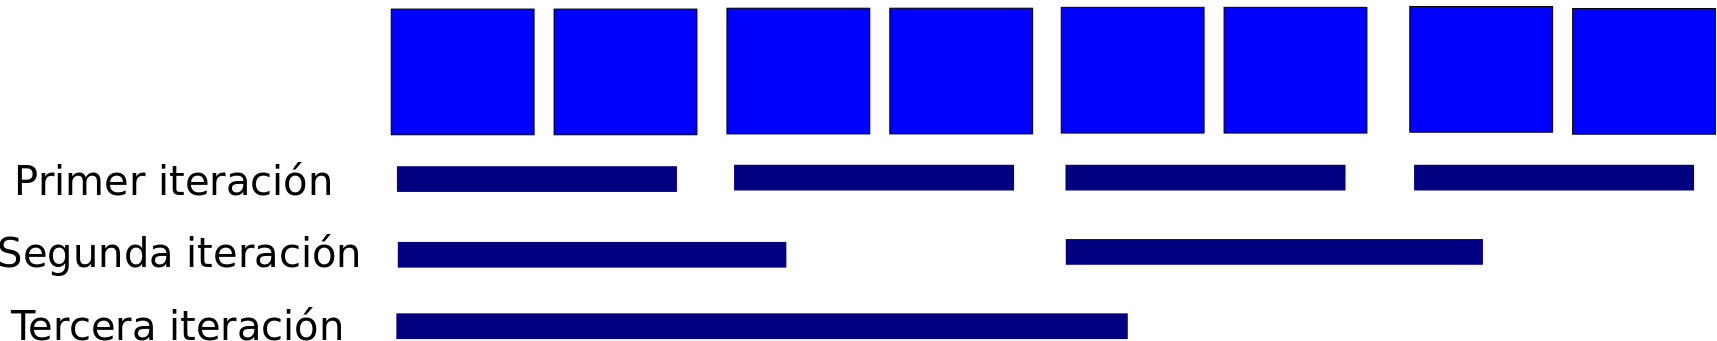
\includegraphics[width=\plotwidth]{images/reductions.png}
   \caption{Esquema de las reducciones realizadas en cada iteraci\'on del ciclo de la
   figura~\ref{code:sum-matrix-bench-code}.}
   \label{fig:sum-matrix-bench-result}
\end{figure}

Claramente este algoritmo debiera producir un mejor tiempo de ejecuci\'on, en
teor\'ia, utilizando m\'ultiples procesadores. Esto suena razonable considerando
que al menos algunas operaciones son delegadas a otros procesadores.

Medimos los tiempos de reducir $128$ matrices de $1024 \times 1024$ elementos de punto
flotante de precisi\'on simple, variando la cantidad de hilos de ejecuci\'on a
utilizar. Para compensar por primeras lecturas y otros factores, se tomo un promedio
de los resultados despu\'es de realizar 20 mediciones sucesivas con la misma
cantidad de \textit{threads}. Todo el c\'odigo se incluye en un ap\'endice de este
trabajo.

Como puede verse en la figura~\ref{fig:sum-matrix-bench-result}, los resultados
son desalentadores: el uso de multiprocesamiento no es \'util para este problema.


\begin{figure}[htbp]
   \centering
   \includegraphics[width=\plotwidth]{plots/cpu/scalability-matrix-sums.png}
   \caption{Tiempo en segundos para sumar 128 matrices de $1024 \times 1024$
   elementos, seg\'un la cantidad de threads usados. Los resultados corresponden
   a un promedio de 20 corridas, consecutivas para cada cantidad.}
   \label{fig:sum-matrix-bench-result}
\end{figure}

Observando el problema en si, notamos lo siguiente: Cada elemento de las
matrices a sumar es accedido de memoria una \'unica vez y el \'unico computo
realizado con este elemento es una suma con los dem\'as. La relaci\'on entre
lecturas de memoria y operaciones con los datos le\'idos es por lo tanto muy baja.

Observemos adem\'as que, al no utilizarse los datos m\'ultiples veces, cada l\'inea
de datos tiene un \textit{cache miss} asociado (el de la l\'inea donde reside) que
no se ve compensado por uso del mismo mientras reside en cach\'e.

Este tipo de problemas se denomina \textit{memory bound}, ya que la velocidad del
\textit{bus} de memoria y la organizaci\'on de la misma es el factor determinante,
no la capacidad de computo.

Esto implica que, pasado un cierto punto de velocidad de reloj de procesador y
cantidad de n\'ucleos, incrementar estos no produce mejoras apreciables. Esto es
lo que se puede ver en la figura~\ref{fig:sum-matrix-bench-result}.

Ver que ese es el caso en la prueba de concepto realizada requiere herramientas
de an\'alisis m\'as sofisticadas. En nuestro caso utilizamos la herramienta de
c\'odigo abierto \textit{perf}. Esta herramienta usa los contadores de
\textit{performance} que presentamos en las secciones anteriores, para dar estad\'isticas
a nivel arquitectural de la aplicaci\'on y de muy fino detalle, como por
ejemplo cantidad de \textit{cache misses}, \textit{stalls} en el pipeline,
cantidad de \textit{branch mispredictions}, etc.

%TODO(jpdarago): Agregar una introduccion a los contadores de perf

A continuaci\'on se muestran los resultados de correr
un an\'alisis de \textit{perf} para 1 y 12 hilos simult\'aneos en la m\'aquina de
prueba. De inter\'es es el valor de \texttt{stalled-cycles-frontend}. Este valor
corresponde al contador de \textit{performance} \texttt{UOPS\_ISSUED.ANY}. Este
contador registra los eventos en los que el procesador esta \textit{stalleado},
es decir el \textit{pipeline } no avanza pues esta a la espera de datos que
lleguen de memoria principal o un evento similar~\cite{Intel3B}. En este
caso, parece ser que este factor es un limitante extremadamente fuerte

{\footnotesize
\begin{verbatim}
$ perf stat -B ./benchmark 1024 128 1
1 0.180418953613844

 Performance counter stats for './benchmark 1024 128 1':

       2076,031257 task-clock                #    0,998 CPUs utilized
               225 context-switches          #    0,108 K/sec
                 0 cpu-migrations            #    0,000 K/sec
            67.583 page-faults               #    0,033 M/sec
     4.325.757.818 cycles                    #    2,084 GHz
     3.685.447.979 stalled-cycles-frontend   #   85,20% frontend cycles idle
   <not supported> stalled-cycles-backend
     1.801.562.845 instructions              #    0,42  insns per cycle
                                             #    2,05  stalled cycles per insn
       220.639.658 branches                  #  106,280 M/sec
           191.368 branch-misses             #    0,09% of all branches

       2,080571933 seconds time elapsed

$ perf stat -B ./benchmark 1024 128 12
12 0.182727314613294

 Performance counter stats for './benchmark 1024 128 12':

      22160,476291 task-clock                #   10,531 CPUs utilized
             2.402 context-switches          #    0,108 K/sec
                17 cpu-migrations            #    0,001 K/sec
            66.704 page-faults               #    0,003 M/sec
    46.310.011.626 cycles                    #    2,090 GHz
    42.797.073.792 stalled-cycles-frontend   #   92,41% frontend cycles idle
   <not supported> stalled-cycles-backend
     9.369.677.336 instructions              #    0,20  insns per cycle
                                             #    4,57  stalled cycles per insn
     2.657.329.767 branches                  #  119,913 M/sec
           687.016 branch-misses             #    0,03% of all branches

       2,104317579 seconds time elapsed
\end{verbatim}
}

Esto lleva a concluir que esta operaci\'on final impactar\'ia muy
negativamente en la escalabilidad de la implementaci\'on, y que por lo tanto a
medida que la cantidad de procesadores se incrementara esta secci\'on del
c\'odigo se har\'ia mucho m\'as pesada. Por lo tanto, se busc\'o reorganizar
este ciclo para no necesitar una matriz separada.

El ciclo a modificar esta en la figura~\ref{fig:rmm.output-previous}.
Se ve f\'acilmente que esto es posible si se invierten los ciclos del algoritmo en
el algoritmo, para poder dividir los \'indices de la matriz global entre m\'ultiples
hilos de ejecuci\'on.

\begin{algorithm}[H]
    \centering
    \label{algo:rmm-output-previous}
    \caption{C\'alculo original de la matriz de Kohn-Sham}
    \begin{algorithmic}
        \State $R \gets 0_{m,n}$
        \State $F \gets functions(PG)$
        \ForAll{$p \in points(PG)$}
            \ForAll{$i,j \in m \times n$}
            \State $R_{i,j} \gets R_{i,j} + F_{p,i} \cdot F_{p,j} \cdot factors_{p}$
            \EndFor
        \EndFor
        \ForAll{$i,j \in fock\_indexes(PG)$}
            \State $KS_{i,j} \gets KS_{i,j} + R_{i,j}$
        \EndFor
    \end{algorithmic}
\end{algorithm}

La versi\'on modificada puede verse en la figura~\ref{fig:rmm-output-new}. Lo que
se hace para este caso es recorrer los \'indices a actualizar de la matriz total
y luego obtener la contribuci\'on de todos los puntos. Dado que cada \'indice debe
ser actualizado por, a lo sumo, un solo hilo de ejecuci\'on, no hay necesidad de
clonar matrices y reducirlas.

\begin{algorithm}[H]
    \centering
    \label{algo:rmm-output-new}
    \caption{C\'alculo de la matriz de Kohn-Sham reestructurado para paralelismo}
    \begin{algorithmic}
        \State $R \gets 0_{m,n}$
        \State $F \gets functions(PG)^T$
        \ForAll{$i,j \in indexes$}
            \State $KS_{i,j} \gets KS_{i,j} + \displaystyle \Sigma_{p \in points(PG)} F_{p,i} \cdot F_{p,j} \cdot factors_{p}$
        \EndFor
    \end{algorithmic}
\end{algorithm}

Un problema provocado por la implementaci\'on es que recorre la matriz de funciones
en orden de columnas, en lugar de orden por filas. Este orden es poco amigable
para los caches ya que cada fila de la matriz probablemente resida en l\'ineas de
cach\'e diferentes. Esto puede disminuir apreciablemente la performance del algoritmo.
Adem\'as, lastima su escalabilidad en procesadores, al incrementarse la cantidad de
invalidaciones de cach\'e y por lo tanto el \textit{overhead} del algoritmo de
coherencia entre caches intreprocesadores.

La soluci\'on a este problema es sin embargo sencilla, trasponiendo la matriz de
valores de funciones. La misma puede trasponerse una vez y almacenarse en memoria
RAM al iniciar las iteraciones, teniendo por lo tanto un relativo bajo costo de
creaci\'on, y el impacto que tiene en la cantidad de \textit{misses} de cach\'e.

Esta modificaci\'on del algoritmo introduce un nuevo aspecto a considerar, similar
a las consideraciones hechas para la cantidad de puntos y funciones: una poca
cantidad de \'indices a actualizar en un mismo grupo eclipsa el \textit{overhead}
que introduce el uso de OpenMP. La cantidad de \'indices de la matriz de Kohn-Sham a
actualizar tambi\'en tiene una distribuci\'on bastante dispar, como puede verse
para el caso de ejemplo de hemoglobina en la figura~\ref{fig:histogram-indexes-hemo}.

\begin{figure}[htbp]
   \centering
   \includegraphics[width=\plotwidth]{plots/cpu/histogram-indexes-hemo.png}
   \caption{Cantidad de \'indices a actualizar de la matriz de Kohn-Sham}
   \label{fig:histogram-indexes-hemo}
\end{figure}

Esto enfatiza a\'un m\'as la necesidad de utilizar una paralelizaci\'on h\'ibrida
para grupos chicos y grandes, ya que ahora se tiene un factor m\'as que determina
cuanto trabajo se le asigna a los \textit{threads}.

Estos dos factores se tienen en cuenta en la funci\'on que determina si un grupo
es considerado grande o no. Para considerar un grupo grande, el mismo debe tener
una cantidad de puntos y una cantidad de \'indices en la matriz de Kohn-Sham mayor que
un valor de frontera (\textit{threshold}) multiplicado por la cantidad de hilos de
ejecuci\'on a realizar. Este valor es ajustable y mostraremos los resultados
correspondientes a tomar la mejor elecci\'on, siendo interesante su efecto en el
tiempo de ejecuci\'on de la iteraci\'on.

\subsection{Algoritmo de balanceo}

Por \'ultimo, si bien el algoritmo de particionado y la funci\'on de costo son
buenas para los casos estudiados, no son perfectas. Como puede verse en la
figura~\ref{fig:lio-imbalance-between-loads}, hay una diferencia entre cargas
no despreciable en algunos casos, con lo cual todav\'ia se puede obtener algo de
mejoras en \textit{performance} entre iteraciones utilizando balanceo de cargas,
que obtuvo buenos resultados en la implementaci\'on para GPGPUS.

\begin{figure}[htbp]
   \centering
   \includegraphics[width=\plotwidth]{plots/cpu/group-split-differences.png}
   \caption{Comparaci\'on de los tiempos de ejecuci\'on para las distintas
   cargas asignadas a cada hilo de ejecuci\'on en el caso de la hemoglobina.}
   \label{fig:lio-imbalance-between-loads}
\end{figure}

El algoritmo es muy similar, se mide el tiempo de \textit{runtime} para cada
grupo de cada carga, y cuanto dura cada una de ellas. Luego, se repite una
cantidad de veces (5 veces, como la implementaci\'on de balanceo en multiplaca)
que se mueve una cierta cantidad de grupos desde la carga m\'as pesada a la
m\'as liviana, de manera de no pasarse de la diferencia temporal que hay entre
ellas. Una vez movidos los grupos correspondientes, y tal que la diferencia
entre los dos estimativos es menor que el 5\% del peso total de la carga m\'as
pesada, se prosigue por encontrar las otras dos cargas m\'as dispares y
rebalancearlas. Para m\'as detalles del algoritmo puede verse la secci\'on
de balanceo de cargas de la implementaci\'on en GPU.

El costo computacional ya se vi\'o anteriormente que resulta bajo. En el caso
de la hemoglobina se consigue menos del 5\% de diferencia en una iteraci\'on
de rebalanceo, obteniendose los resultados de la figura~\ref{fig:lio-imbalance-fixed}.

\begin{figure}[htbp]
   \centering
   \includegraphics[width=\plotwidth]{plots/cpu/group-split-differences-post-balance.png}
   \caption{Comparaci\'on de los tiempos de ejecuci\'on para las distintas
   cargas asignadas a cada hilo de ejecuci\'on en el caso de la hemoglobina,
   luego de rebalancear}
   \label{fig:lio-imbalance-fixed}
\end{figure}
